\subsection{Ablation of Measure-Aware Physics-Attention}
\label{app:beta_ablation}

Section~\ref{sec:density_consistent_transolver} shows that changing the
inference-time sampling measure changes the limiting point-to-slice
aggregation in Physics-Attention. In particular, when points are sampled
from an adaptive measure $\widetilde{\rho}$ rather than the reference
measure $\rho$, the original Transolver aggregation converges to an
operator under $\widetilde{\rho}$ instead of the reference operator under
$\rho$. The measure-aware aggregation corrects this shift using
$c(x)=\mathrm d\rho/\mathrm d\widetilde{\rho}$.
Here we isolate the practical consequence of this sampling-induced bias:
\emph{with exactly the same adaptively sampled points, how much does an
incorrect measure correction affect inference accuracy?}

Let
\begin{equation}
    \lambda_{\mathrm{eff}}(x)
    =
    \frac{\mathrm d\widetilde{\rho}_{\mathrm{eff}}}
         {\mathrm d\rho}(x)
\end{equation}
denote the effective density ratio represented by the selected samples,
as estimated by the coverage construction in Appendix~\ref{app:density_policy_design}.
The corresponding correction weight is
$c(x)=\lambda_{\mathrm{eff}}(x)^{-1}$.
We temper this correction by an exponent $\beta\in[0,1]$,
\begin{equation}
    c_{\beta}(x)
    =
    c(x)^{\beta}
    =
    \lambda_{\mathrm{eff}}(x)^{-\beta}.
    \label{eq:beta_tempered_correction}
\end{equation}
For self-normalized point-to-slice aggregation, applying
$c_{\beta}$ to samples drawn from $\widetilde{\rho}_{\mathrm{eff}}$
is equivalent, in the population limit, to aggregation under
\begin{equation}
    \mathrm d\rho_{\beta}(x)
    =
    \frac{
        \lambda_{\mathrm{eff}}(x)^{1-\beta}
    }{
        \int_{\Omega}
        \lambda_{\mathrm{eff}}(y)^{1-\beta}
        \,\mathrm d\rho(y)
    }
    \,\mathrm d\rho(x).
    \label{eq:beta_effective_measure}
\end{equation}
Thus, $\beta$ continuously controls the remaining density contrast
relative to the reference measure. At $\beta=0$,
$\rho_{\beta}=\widetilde{\rho}_{\mathrm{eff}}$, recovering the original
Transolver aggregation without density compensation. At $\beta=1$,
$\rho_{\beta}=\rho$, corresponding to full measure correction.
Intermediate values retain a tempered measure shift; equivalently, the
log-density contrast relative to the reference measure is scaled by
$1-\beta$.

The main experiments use the task- and policy-specific correction exponent
$\beta^{\star}$ specified in Appendix~\ref{app:density_policy_design}.
To isolate the effect of measure correction from the effect of adaptive
sampling itself, this ablation does \emph{not} resample points when
$\beta$ changes. For each PI, CPG, and CA policy, we first generate the
coarse and final point sets exactly as in the main experiments. We then
rerun inference on these same point sets while changing only the
correction weights $c_i^{\beta}$ inside the point-to-slice aggregation.
The frozen operator and refinement-head checkpoints, sampled indices,
reconstruction procedure, test examples, and sampling seeds are therefore
identical across all values of $\beta$. We evaluate
$\beta\in\{0,0.25,0.5,0.75,1\}$ at retained fractions of
$37.5\%$, $50\%$, and $75\%$, using sampling seeds 0, 1, and 2.

To summarize the effect across point budgets, let
$A_{m,s}(\beta)$ denote the trapezoidal area under the error--budget
curve for policy $m$ and sampling seed $s$. Figure~\ref{fig:beta_ablation}
reports
\begin{equation}
    R_m(\beta)
    =
    \frac{1}{3}
    \sum_{s=0}^{2}
    \frac{A_{m,s}(\beta)}
         {A_{m,s}(0)}.
    \label{eq:beta_relative_area}
\end{equation}
The normalization is performed separately for each policy and seed before
averaging. Hence $R_m(0)=1$, and $R_m(\beta)<1$ means that measure
correction improves inference over the original, uncompensated
Physics-Attention \emph{on exactly the same adaptive samples}. This
normalization removes the benefit of the sampling locations themselves
and exposes only the effect of correcting their induced measure shift.
Table~\ref{tab:beta_ablation} additionally reports the
Uniform-normalized rAUEC and compares $\beta=0$ with the
main-experiment value $\beta^{\star}$.

\begin{figure}[!htbp]
    \centering
    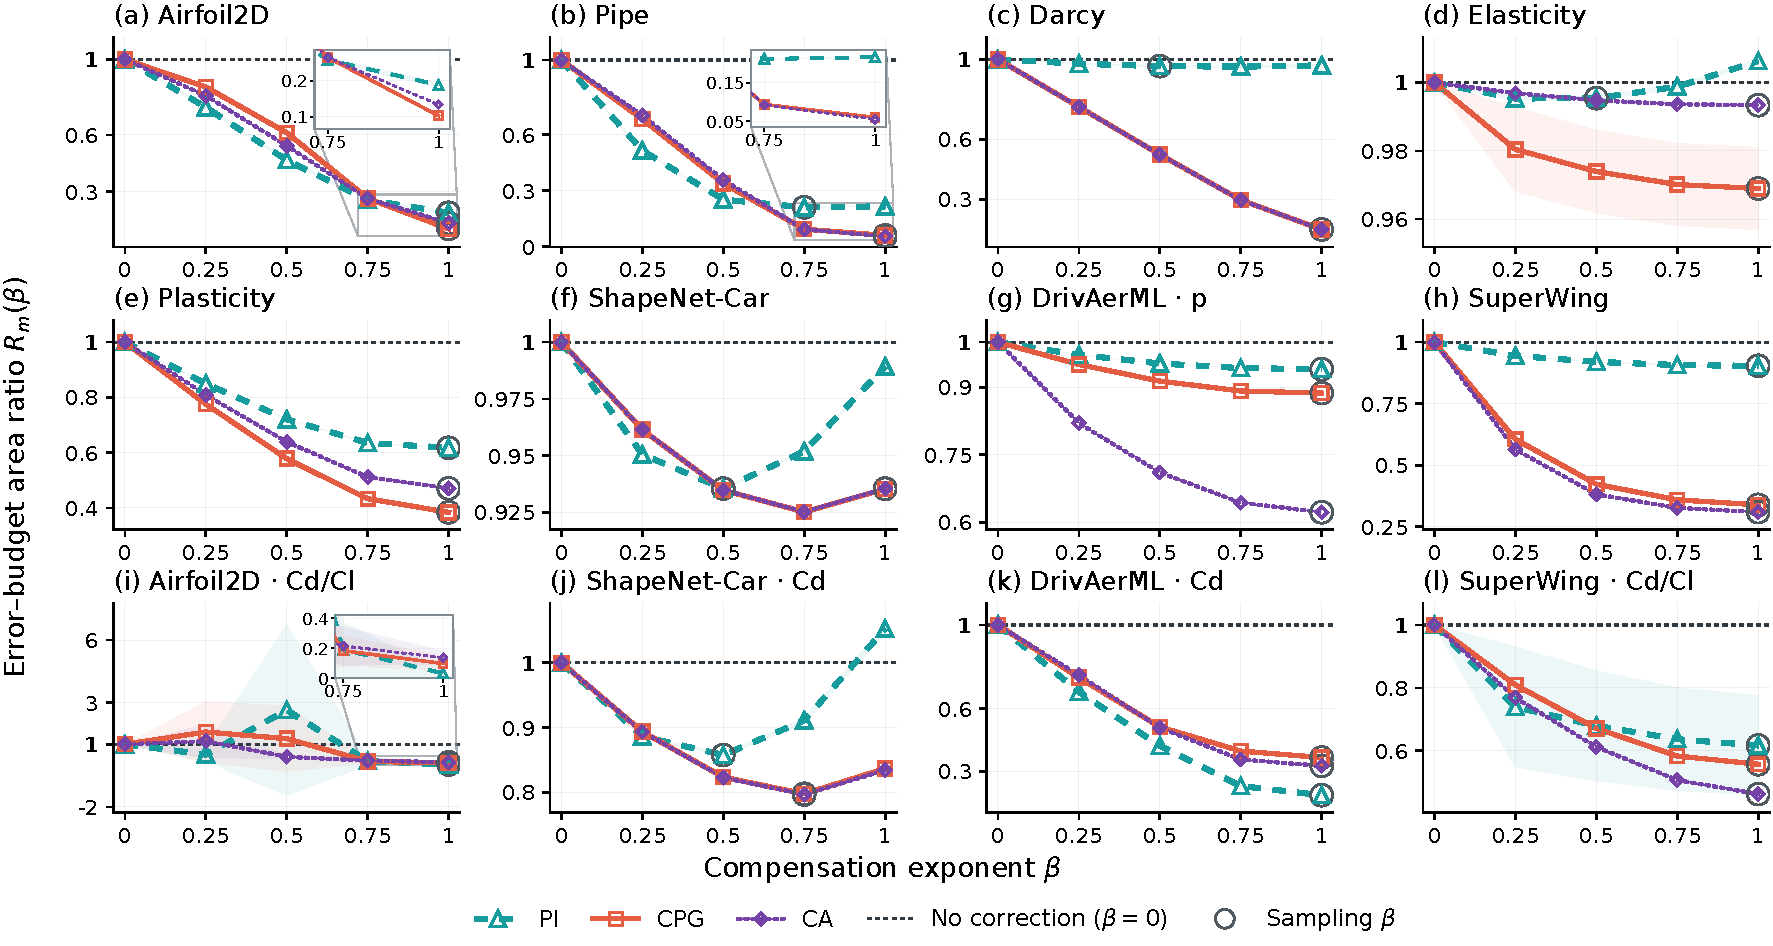
\includegraphics[width=\linewidth]{figures/appendix/beta_ablation.pdf}
\caption{\textbf{Ablation of the measure-correction exponent.}
Checkpoints, sampled points, and reconstruction are fixed. The y-axis is
$R_m(\beta)$ from \eqref{eq:beta_relative_area}: each policy and seed is
normalized to its own $\beta=0$ error--budget area before averaging.
Areas cover $37.5\%$, $50\%$, and $75\%$ budgets. Bands show one sample
standard deviation across three seeds. Gray rings (Sampling $\beta$) mark the
compensation exponent used by each policy in the main experiments.
The dashed line denotes no correction. Insets enlarge high-$\beta$
portions; the Airfoil ratio panel retains the full uncertainty envelope.
Table~\ref{tab:beta_ablation} uses Uniform-normalized rAUEC.}
\label{fig:beta_ablation}
\end{figure}


The results closely follow the measure-shift analysis.
Across most datasets and policies, adaptive sampling without the
corresponding compensation produces substantially larger errors, whereas
moving the correction toward the density associated with the sampler
sharply reduces the error. Because the sampled locations are unchanged,
these improvements cannot be attributed to placing points in better
regions; they arise from correcting how the same point features are
aggregated into physics tokens.

The effect is particularly pronounced when the adaptive density is strongly
non-uniform. For CPG, full correction reduces the error--budget area by
$89.7\%$ on Airfoil field prediction and by $93.9\%$ on Pipe.
On Darcy, the CPG and CA rAUECs decrease from $4.278$ and $4.265$ without
correction to $0.642$ and $0.640$, respectively, even though the sampled
points are identical. Similarly, full correction reduces the SuperWing
field error--budget area by $66.1\%$ for CPG and $69.1\%$ for CA, and
reduces the DrivAerML drag area by $63.3\%$ and $67.3\%$.

\begin{table}[!htbp]
\centering
\small
\caption{Measure correction on fixed adaptive samples. Entries are mean rAUEC over three sampling seeds, with Uniform equal to one. Bold marks the lower value in each within-policy $\beta=0$/$\beta^{\star}$ pair. Parentheses give the percentage decrease in mean rAUEC from $\beta=0$, computed before rounding. The compensation exponents $\beta^{\star}$ are specified in Appendix~\ref{app:density_policy_design}.}
\label{tab:beta_ablation}
\setlength{\tabcolsep}{3pt}
\begin{tabular}{@{}llrrrrrr@{}}
\toprule
Dataset & Metric & \multicolumn{2}{c}{PI} & \multicolumn{2}{c}{CPG} & \multicolumn{2}{c}{CA} \\
\cmidrule(lr){3-4}\cmidrule(lr){5-6}\cmidrule(lr){7-8}
& & $\beta=0$ & $\beta^{\star}$ & $\beta=0$ & $\beta^{\star}$ & $\beta=0$ & $\beta^{\star}$ \\
\midrule
Airfoil & Field & 3.2852 & \textbf{0.6166}\,{\footnotesize (81.2\%)} & 5.6733 & \textbf{0.5831}\,{\footnotesize (89.7\%)} & 4.1829 & \textbf{0.5579}\,{\footnotesize (86.7\%)} \\
Pipe & Field & 4.1234 & \textbf{0.8711}\,{\footnotesize (78.9\%)} & 11.1004 & \textbf{0.6719}\,{\footnotesize (93.9\%)} & 12.7244 & \textbf{0.7051}\,{\footnotesize (94.5\%)} \\
Darcy & Field & 1.0315 & \textbf{0.9965}\,{\footnotesize (3.4\%)} & 4.2778 & \textbf{0.6419}\,{\footnotesize (85.0\%)} & 4.2654 & \textbf{0.6400}\,{\footnotesize (85.0\%)} \\
Elasticity & Field & 0.7314 & \textbf{0.7280}\,{\footnotesize (0.5\%)} & 0.4832 & \textbf{0.4681}\,{\footnotesize (3.1\%)} & 0.5506 & \textbf{0.5469}\,{\footnotesize (0.7\%)} \\
Plasticity & Field & 1.4393 & \textbf{0.8888}\,{\footnotesize (38.2\%)} & 2.3153 & \textbf{0.8890}\,{\footnotesize (61.6\%)} & 1.8908 & \textbf{0.8897}\,{\footnotesize (52.9\%)} \\
ShapeNet-Car & Field & 0.6301 & \textbf{0.5895}\,{\footnotesize (6.4\%)} & 0.5962 & \textbf{0.5577}\,{\footnotesize (6.5\%)} & 0.5962 & \textbf{0.5577}\,{\footnotesize (6.4\%)} \\
DrivAerML & Field & 0.9398 & \textbf{0.8834}\,{\footnotesize (6.0\%)} & 0.9298 & \textbf{0.8246}\,{\footnotesize (11.3\%)} & 1.3280 & \textbf{0.8263}\,{\footnotesize (37.8\%)} \\
SuperWing & Field & 0.8369 & \textbf{0.7564}\,{\footnotesize (9.6\%)} & 1.9796 & \textbf{0.6706}\,{\footnotesize (66.1\%)} & 2.3252 & \textbf{0.7193}\,{\footnotesize (69.1\%)} \\
Airfoil & Cd/Cl & 11.3964 & \textbf{0.2174}\,{\footnotesize (98.1\%)} & 2.1147 & \textbf{0.2379}\,{\footnotesize (88.7\%)} & 1.7583 & \textbf{0.2453}\,{\footnotesize (86.1\%)} \\
ShapeNet-Car & Cd & 0.7649 & \textbf{0.6561}\,{\footnotesize (14.2\%)} & 0.8113 & \textbf{0.6474}\,{\footnotesize (20.2\%)} & 0.8130 & \textbf{0.6479}\,{\footnotesize (20.3\%)} \\
DrivAerML & Cd & 4.9553 & \textbf{0.9245}\,{\footnotesize (81.3\%)} & 2.5121 & \textbf{0.9209}\,{\footnotesize (63.3\%)} & 2.8282 & \textbf{0.9244}\,{\footnotesize (67.3\%)} \\
SuperWing & Cd/Cl & 1.4093 & \textbf{0.8246}\,{\footnotesize (41.5\%)} & 1.4403 & \textbf{0.8026}\,{\footnotesize (44.3\%)} & 1.7669 & \textbf{0.8167}\,{\footnotesize (53.8\%)} \\
\bottomrule
\end{tabular}
\end{table}


More generally, the minima of the curves occur at or near the correction
strength used by the corresponding sampling policy in the main
experiments. When the effective density is well represented by the
coverage estimate, the lowest error is typically attained close to full
correction. When a tempered correction is used in the main policy, the
preferred exponent shifts accordingly; for example,
ShapeNet-Car drag attains its lowest area near
$\beta^{\star}=0.75$ for CPG and CA. Conversely, moving the compensation
profile away from that associated with the sampler generally increases
the inference error.

These results provide a direct empirical test of the bias characterized
in Section~\ref{sec:density_consistent_transolver}. Adaptive sampling
changes not only \emph{where} the operator is evaluated, but also the
measure under which point features are aggregated. Keeping the samples
fixed while perturbing only the compensation weights reproduces the
predicted degradation: the larger the mismatch between the sampling
measure and the measure used in aggregation, the larger the resulting
inference bias. Measure-aware Physics-Attention is therefore necessary
to separate adaptive spatial allocation from an unintended change of the
operator being evaluated.